\section{Experiment 1: Sentence-level vs Word-level Quality}

Consistent with our proposed novel design process, a main goal of this user study is to identify what underdeveloped XAI methods might be useful to users and thus are worth further refining. To achieve this end we test two different types of MT XAI - sentence level quality score, and word-level predicted errors. In addition, we anticipate differences in passages will play a role in users’ performance. Thus we include two different passage types in this study for balance. This results in a 4 condition experiment. Examples of stimuli are shown in Figure \ref{fig:exp1_stim}. In the experiment participants were shown 4 passages of 3 sentences. Before being asked to answer simple questions about a passage, participants were given the opportunity to request a human re-translation of any one sentence in a passage. In the following sections we outline this study in more detail. 

\subsection{XAI Techniques} 

\ab{need to make sure this connects to where we talk about VeriCAT earlier.} There are two main methods for estimating MT quality: \ab{is this right? I feel like I might have made it up} sentence-level quality estimations, and word-level error predictions. 
%Currently, quality estimation models for sentence-level quality far outperform word-level error prediction models. In line with our novel XAI design approach, we test both of these methods with the belief that if we find word-level estimations significantly improve users performance in identifying poorly translated snippets, then there is an impetus for further refinement of word-level error prediction models. 
Neither of these models is perfect so for the sake of the design process we test idealized versions of each. 

\begin{compacthang}
    \item \textbf{Sentence-level quality scores} These scores range from 0 to 100 with 0 indicating a poor quality translation, and 100 indicating a perfect translation. Scores are shown to users as percentages and progress bars, as shown in Figures \ref{fig:p3_quality} and \ref{fig:p4_markup_quality}. We included only sentences with clearly good (> 70) or poor (< 30) quality scores, and used scores generated by humans \ab{need to add correct name}. We included only scores above 70 or below 30 to avoid the confounding factor of no clear difference between high and low sentence-level quality estimations. And we used human generated quality scores, because predicted scores are not sufficiently varied as high and low. In the case that sentence-level quality scores significantly increase participants’ performance, we would encourage further development of predicted scores that simulate human scores. 

    \item \textbf{Word-level error predictions} These predictions predict missing, incorrect, and extra words in a MT. They are shown to users via red `\textcolor{red}{\_}''s for missing words, and \textcolor{red}{red highlighting} for incorrect and extra words, as shown in Figures \ref{fig:p2_markup} and \ref{fig:p4_markup_quality}. To avoid the confounding factor of accuracy of the word-level prediction model, we identified all word-level errors by hand based on human translations. In the case that word-level error prediction significantly increases participants’ performance, we would encourage further development of word-level error predictions that are very close to ground truth.  
\end{compacthang}

\subsection{Passage Type}
We postulate that without an XAI users will rely on fluency as a proxy for translation quality. Prior work has shown that this is the case when it comes to trust of MT \cite{martindaleFluency2018}. However, there are cases where this technique fails. For example, sentences written in ALL CAPS are notoriously difficult for MT, and often what they are translated is inaccurate but deceptively fluent. 

Each sentence can fall into one of four categories: poor fluency + poor quality, poor fluency + good quality, good fluency + poor quality, good fluency + good quality. Of these, we expect  sentences in the good fluency + poor quality, and poor fluency + good quality categories to be the most difficult for participants to assess. To test if these different sentence types have an effect on participants’ performance we arrange two different types of passages. 

\begin{compacthang}
    \item \textbf{Type 1} Good fluency + good quality, good fluency + poor quality, poor fluency + good quality. In this passage type we expect participants assigned to baseline (no XAI) to select the poor fluency sentence for re-translation. This passage type is designed to test if participants in an XAI condition will follow the quality indicators shown by the XAI to select a sentence for re-translation, or if they will also use fluency to decide. Passages 1 and 2 as shown in Figures \ref{fig:p1_no_xai} and \ref{fig:p2_markup} are of this type.    

    \item \textbf{Type 2} Good fluency + good quality, poor fluency + good quality, poor fluency + poor quality. In this passage type we expect participants assigned to baseline (no XAI) to select one of the poor fluency sentences for re-translation. This passage type is designed to test if participants in an XAI condition will follow the quality indicators shown by the XAI to select a sentence for re-translation (particularly because it should help them choose which poor fluency sentence to select), or if they will also use fluency to decide. Passages 1 and 2 as shown in Figures \ref{fig:p3_quality} and \ref{fig:p4_markup_quality} are of this type.     
\end{compacthang}

\begin{figure}
    \centering
    \begin{subfigure}[t]{0.45\textwidth}
        \centering
        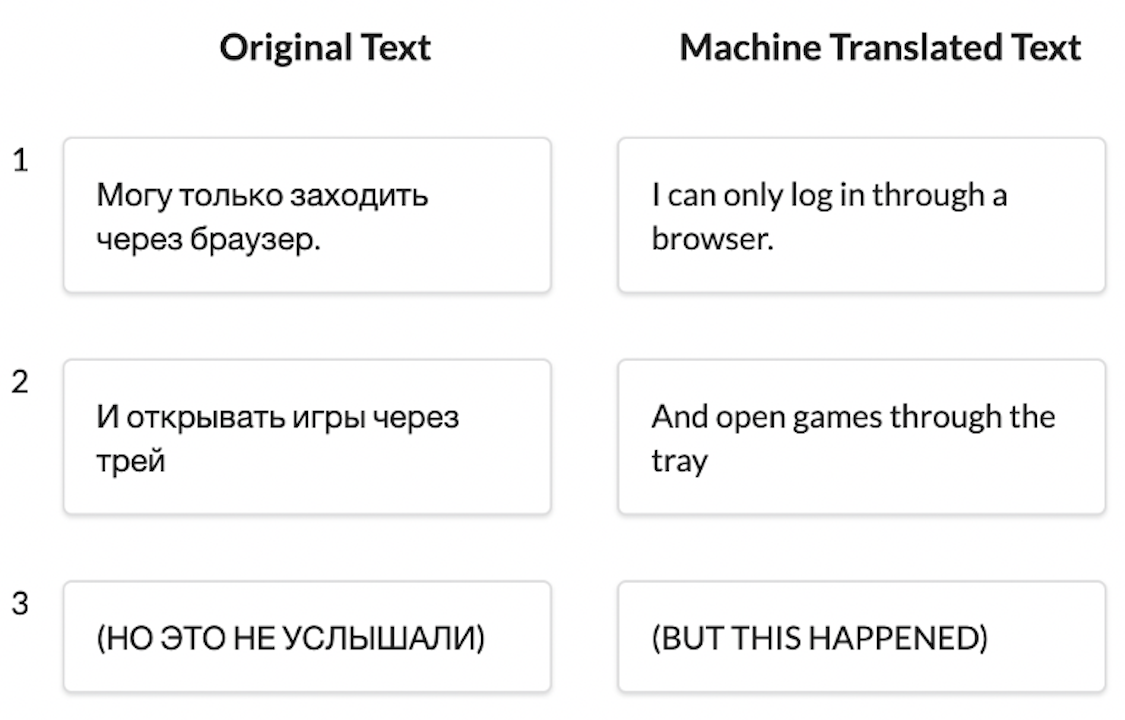
\includegraphics[width=\linewidth]{p1_c_0.png} 
        \caption{Passage 1 (passage type 1), No XAI condition} \label{fig:p1_no_xai}
    \end{subfigure}
    \hfill
    \begin{subfigure}[t]{0.45\textwidth}
        \centering
        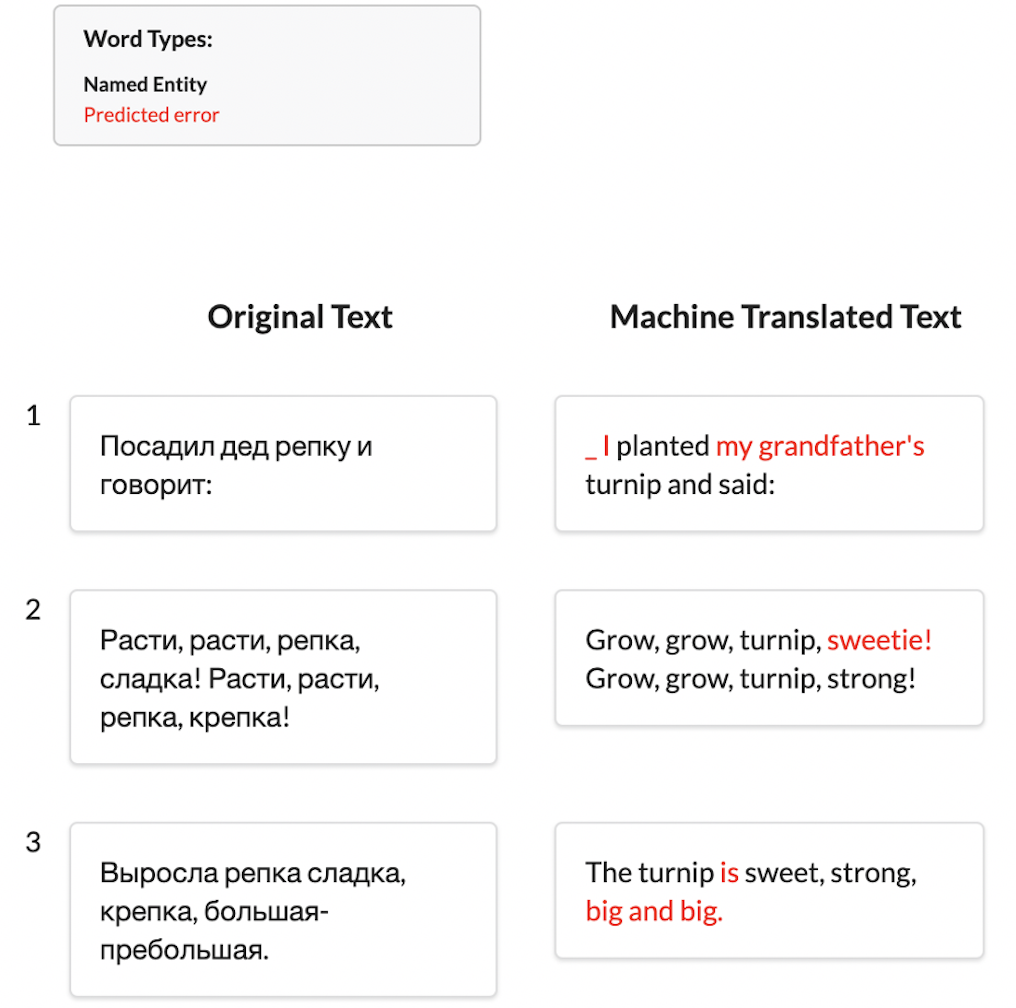
\includegraphics[width=\linewidth]{p2_m_0.png} 
        \caption{Passage 2 (passage type 1), Markup condition} \label{fig:p2_markup}
    \end{subfigure}
    
    \vspace{5px}
    
     \begin{subfigure}[t]{0.45\textwidth}
        \centering
        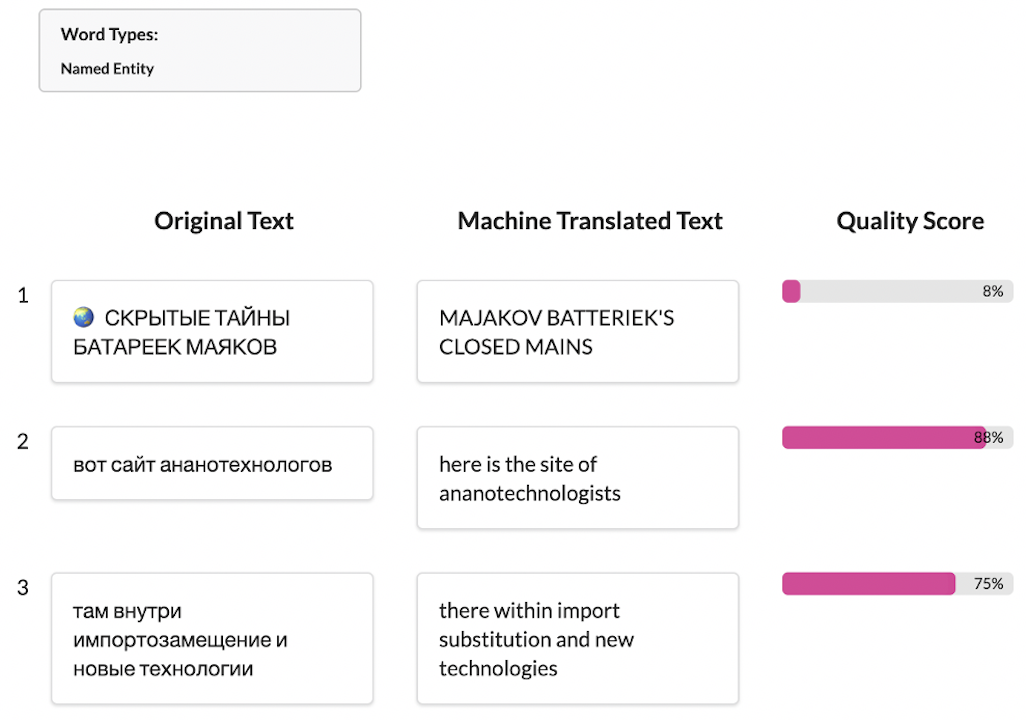
\includegraphics[width=\linewidth]{p3_v_0.png} 
        \caption{Passage 3 (passage type 2), Quality condition} \label{fig:p3_quality}
    \end{subfigure}
    \hfill
    \begin{subfigure}[t]{0.45\textwidth}
        \centering
        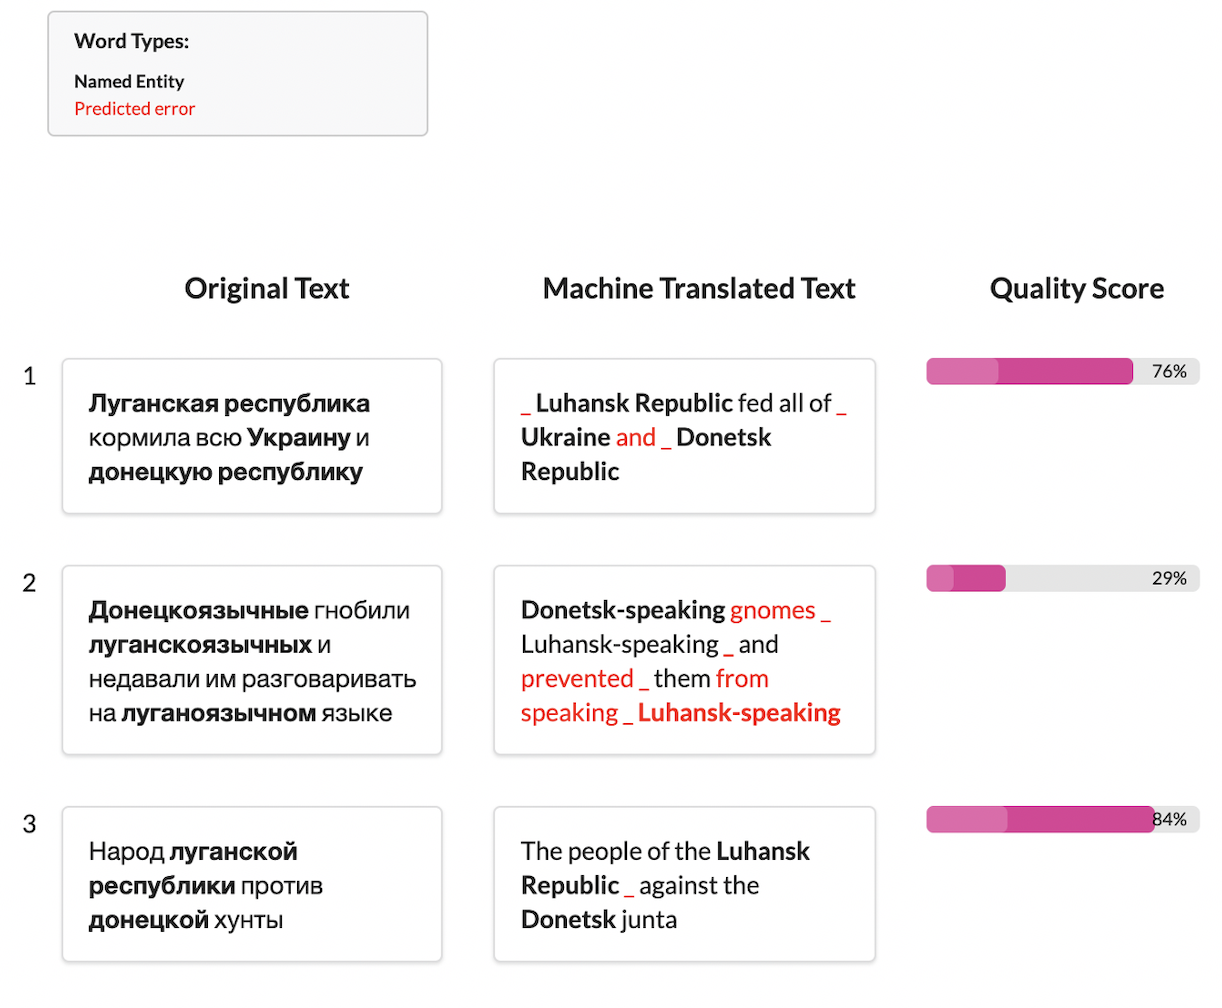
\includegraphics[width=\linewidth]{p4_mq_0.png} 
        \caption{Passage 4 (passage type 2), Markup+Quality condition} \label{fig:p4_markup_quality}
    \end{subfigure}
    
    \caption{Select examples of stimuli for Experiment 1. All stimuli are available in supplemental materials.}
    \label{fig:exp1_stim}
    
\end{figure}

\subsection{Task} 
We ran a 4 condition experiment. Each condition consists of a different XAI technique, and within each condition we include 2 different passage types. The experimental task aimed to replicate the Facebook “Does this need a human translation?” situation as closely as possible within a controlled setting. Therefore, for the task we ask users to look at a passage of text (comprised of 3 sentences), decide if any of the sentences in the passage should be re-translated by a human, and then answer 2 information retrieval questions based on the passage. This repeated for 4 passages; two of type 1 followed by two of type 2. The prompt before each passage was as follows:

\begin{quote}
Below is a passage written in Russian with an English translation generated by artificial intelligence. When you are ready, you will be asked to answer two comprehension questions. \textbf{You may select up to one section of the passage for re-translation by a human.} We recommend selecting the section you judge to have the poorest machine translation for re-translation by a human. 

Click ``I’m ready to see the questions'' when you are ready to see the comprehension questions. \textbf{If you would like a human re-translation of any section of the passage you must request it BEFORE you click ``I’m ready to see the questions''.} Once you click ``I’m ready to see the questions'', comprehension questions will appear on the page alongside the Russian test, English Machine translation, and any human translations you requested.  
\end{quote}

Participants were then given the chance to select sentence 1, 2, or 3 of the passage for re-translation by a human, or no-retranslation. After their selection the original passage and machine translation remained on the screen in addition to the human translation of whichever sentence they selected for re-translation, and two information retrieval questions.  

\begin{table}[]
\resizebox{0.80\textwidth}{!}{%
\begin{tabular}{c|c|c|c}
\hline
\begin{tabular}[c]{@{}c@{}}Quality Score XAI\\ (Quality)\end{tabular} & \begin{tabular}[c]{@{}c@{}}Word-level Markup XAI\\ (Markup)\end{tabular} & \begin{tabular}[c]{@{}c@{}}Word-level Markup + Quality XAI\\ (Markup+Quality)\end{tabular} & \begin{tabular}[c]{@{}c@{}}No XAI\\ (No XAI)\end{tabular} \\ \hline
69                                                                    & 55                                                                       & 49                                                                                         & 47                                                        \\ \hline
\end{tabular}
}
\caption{N for each condition in Experiment 1. }
\label{tab:exp1_N}
\end{table}


\subsection{Participants} 

We recruited 256 participants from Amazon Mechanical Turk. Participation was restricted to
workers in the United States with an approval rating of greater than 90 percent. Participants were paid a base rate of USD $1.60$ for participation. Before analysis, participants who answered information retrieval questions for passage 1 and passage 2 incorrectly (which were attention check questions) were dropped from analysis ($N = 46$).  This left $N = 210$ participants distributed among stimuli as shown in Table \ref{tab:exp1_N}. Demographics of participants are shown in Table \ref{tab:exp1_demo}.


\begin{table}[h!]
\begin{threeparttable}[b]
\begin{tabular}{ll}
\hline
N                                                                                & 210                                                                                                                                                    \\ \hline
Age                                                                              & \begin{tabular}[c]{@{}l@{}}18-24: 6.2\%, 25-34: 45.2\%, 35-44: 26.2\%, \\ 45-54: 12.9\%, 55-64: 7.6\%, 65+: 4.4\%\end{tabular}                                     \\ \hline
Gender                                                                           & \begin{tabular}[c]{@{}l@{}}Female: 30.5\%, Male: 69.0\%\end{tabular}                                                             \\ \hline
Education                                                                        & \begin{tabular}[c]{@{}l@{}}High School: 16.2\%, Associates: 8.6\%, Bachelors: 56.7\%, \\ Masters: 15.2\%, Professional: 1.9\%, Other: 1.0\%\end{tabular}                            \\ \hline
\end{tabular}
\end{threeparttable}
\caption{Participant demographics for Experiment 1.}
\label{tab:exp1_demo}
\end{table}

\subsection{Procedure}

The experiment followed an approved protocol per redacted for anonymity’s company policy, and was posted as a HIT on Amazon Mechanical Turk. Workers who accepted the HIT followed a link to the experiment. After providing informed consent, participants were taken to an instruction page explaining the experiment. This page explained that they would see 4 passages of text translated from Russian to English by AI. They were told that they would be asked to answer two comprehension questions for each passage, but before doing so would have the opportunity to see one of the sentences in the passage re-translated by a human. After the instruction page, participants were shown the four passages one at a time. Participants could take as much time with each stimulus as they wanted before clicking a button to select which section of the passage they wanted re-translated by a human and viewing the questions to answer. After completing the main task participants were asked to complete a short post-experiment questionnaire, the Tolerance for Ambiguity Survey from Geller et al. 1993 \cite{gellerTolerance1993}, a short demographic questionnaire, and to provide any additional feedback they wished.

\subsection{Hypotheses}

%We postulate that adding XAI to machine translations of text will help users identify poorly translated sentences, particularly in cases where the poor translations have good fluency. However, we anticipate that too much explanation will overwhelm users and detract significantly from the efficacy of XAI.

To evaluate the VeriCAT system with Word- vs. Sentence-level Quality Scores, we test the following hypotheses:

\begin{compacthang}
    \item \textbf{H1.1}: Participants in the XAI conditions will have higher accuracy in identifying which sentence in a passage is of low quality and should be re-translated than participants in the No XAI condition. 
    \item \textbf{H1.2}: Participants in the Quality Score + Word-level Markup (Quality+Markup) condition will have lower accuracy than participants in the Quality and Markup conditions. 
    \item \textbf{H2.1}: There will be a significantly greater change in trust of machine translation for participants in an XAI condition than for users in the No XAI condition. 
    \item \textbf{H3.1}: Participants’ tolerance for ambiguity will correlate with how well they are able to use XAI to perform the experimental task. 
    \item \textbf{H3.2}: Participants’ experience using machine translation will correlate with how well they are able to use XAI to perform the experimental task. 
    \item \textbf{H3.3}: Participants’ self-rated expertise in AI, MT, visualization, and statistics will correlate with how well they are able to use XAI to perform the experimental task.   
\end{compacthang}

\subsection{Findings}

We considered a participant’s answer correct if they selected the sentence in a passage with the lowest quality score as the one to get re-translated by a human. To calculate overall accuracy, we summed the number of correct answers across all four passages and divided by 4. The following analyses use this outcome measure to test the hypotheses listed above.

\subsubsection{Does XAI help?}

We start by looking at which sentences people chose to re-translate for each condition and passage. For all  passages we see participants in the Quality condition are on average most accurate at selecting the correct sentence for re-translation. Interestingly, we see that participants in the No XAI condition tend to opt for no-retranslation, or re-translating a poor fluency sentence. Participants in the Markup+Quality condition tend to select correctly, but not in as high proportions as participants in the Quality condition. Finally, people in the Markup condition surprisingly tend to behave similar to the No XAI condition and choose no re-translation almost as often as they choose the correct sentence. Proportions of participants giving each answer for each passage and condition are shown in Figure \ref{fig:exp1_prop_answers}.

\begin{figure}[h!]
    \centering
    
    \cbox{bar-noXai} \textit{No XAI} \quad
    \cbox{bar-Qual} \textit{Quality} \quad
    \cbox{bar-Markup} \textit{Markup} \quad
    \cbox{bar-MarkupQ} \textit{Markup$+$Quality}
    
    \begin{subfigure}[t]{0.45\textwidth}
        \centering
        \scalebox{0.7}{
        \begin{bchart}[step=.25,max=1,width=\linewidth]
        \bcbar[color=bar-noXai]{.06}
        \bcbar[color=bar-Qual]{.51}
        \bclabel{\textit{Good Fluency}}
        \bcbar[color=bar-Markup]{.35}
        \bclabel{\textit{Poor score}}
        \bcbar[color=bar-MarkupQ]{.43}
        \bcskip{6pt}
        
        \bcbar[color=bar-noXai]{.15}
        \bcbar[color=bar-Qual]{.15}
        \bclabel{\textit{Good Fluency}}
        \bcbar[color=bar-Markup]{.09}
        \bclabel{\textit{Good score}}
        \bcbar[ color=bar-MarkupQ]{.14}
        \bcskip{6pt}
        
        \bcbar[color=bar-noXai]{.38}
        \bcbar[color=bar-Qual]{.14}
        \bclabel{\textit{Poor Fluency}}
        \bcbar[color=bar-Markup]{.24}
        \bclabel{\textit{Good score}}
        \bcbar[ color=bar-MarkupQ]{.22}
        \bcskip{6pt}
        
        \bcbar[color=bar-noXai]{.40}
        \bcbar[color=bar-Qual]{.20}
        \bclabel{\textit{No}}
        \bcbar[color=bar-Markup]{.33}
        \bclabel{\textit{Re-translation}}
        \bcbar[ color=bar-MarkupQ]{.20}
        
        \bcxlabel{Proportion of Participants Selecting}
        \end{bchart}}
        \caption{Passage 1} 
        \label{fig:exp1_p1_prop_answers}
    \end{subfigure}
    \hfill
    \begin{subfigure}[t]{0.45\textwidth}
        \centering
        \scalebox{0.7}{
        \begin{bchart}[step=.25,max=1,width=\linewidth]
        \bcbar[color=bar-noXai]{.06}
        \bcbar[color=bar-Qual]{.53}
        \bclabel{\textit{Good Fluency}}
        \bcbar[color=bar-Markup]{.13}
        \bclabel{\textit{Poor score}}
        \bcbar[ color=bar-MarkupQ]{.41}
        \bcskip{6pt}
        
        \bcbar[color=bar-noXai]{.13}
        \bcbar[color=bar-Qual]{.12}
        \bclabel{\textit{Good Fluency}}
        \bcbar[color=bar-Markup]{.18}
        \bclabel{\textit{Good score}}
        \bcbar[ color=bar-MarkupQ]{.12}
        \bcskip{6pt}
        
        \bcbar[color=bar-noXai]{.21}
        \bcbar[color=bar-Qual]{.15}
        \bclabel{\textit{Poor Fluency}}
        \bcbar[color=bar-Markup]{.22}
        \bclabel{\textit{Good score}}
        \bcbar[color=bar-MarkupQ]{.29}
        \bcskip{6pt}
        
        \bcbar[color=bar-noXai]{.60}
        \bcbar[color=bar-Qual]{.20}
        \bclabel{\textit{No}}
        \bcbar[color=bar-Markup]{.47}
        \bclabel{\textit{Re-translation}}
        \bcbar[color=bar-MarkupQ]{.18}
        
        \bcxlabel{Proportion of Participants Selecting}
        \end{bchart}}
        \caption{Passage 2} 
        \label{fig:exp1_p2_prop_answers}
    \end{subfigure}
    \hfill
     \begin{subfigure}[t]{0.45\textwidth}
        \centering
        \scalebox{0.7}{
        \begin{bchart}[step=.25,max=1,width=\linewidth]
        \bcbar[color=bar-noXai]{.26}
        \bcbar[color=bar-Qual]{.69}
        \bclabel{\textit{Poor Fluency}}
        \bcbar[color=bar-Markup]{.38}
        \bclabel{\textit{Poor score}}
        \bcbar[color=bar-MarkupQ]{.53}
        \bcskip{6pt}
        
        \bcbar[color=bar-noXai]{.19}
        \bcbar[color=bar-Qual]{.05}
        \bclabel{\textit{Poor Fluency}}
        \bcbar[color=bar-Markup]{.20}
        \bclabel{\textit{Good score}}
        \bcbar[color=bar-MarkupQ]{.12}
        \bcskip{6pt}
        
        \bcbar[color=bar-noXai]{.09}
        \bcbar[color=bar-Qual]{.10}
        \bclabel{\textit{Good Fluency}}
        \bcbar[color=bar-Markup]{.09}
        \bclabel{\textit{Good score}}
        \bcbar[color=bar-MarkupQ]{.18}
        \bcskip{6pt}
        
        \bcbar[color=bar-noXai]{.47}
        \bcbar[color=bar-Qual]{.15}
        \bclabel{\textit{No}}
        \bcbar[color=bar-Markup]{.33}
        \bclabel{\textit{Re-translation}}
        \bcbar[color=bar-MarkupQ]{.16}
        
        \bcxlabel{Proportion of Participants Selecting}
        \end{bchart}}
        \caption{Passage 3} 
        \label{fig:exp1_p3_prop_answers}
    \end{subfigure}
    \hfill
    \begin{subfigure}[t]{0.45\textwidth}
        \centering
        \scalebox{0.7}{
        \begin{bchart}[step=.25,max=1,width=\linewidth]
        \bcbar[color=bar-noXai]{.45}
        \bcbar[color=bar-Qual]{.64}
        \bclabel{\textit{Poor Fluency}} 
        \bcbar[color=bar-Markup]{.58}
        \bclabel{\textit{Poor score}}
        \bcbar[color=bar-MarkupQ]{.57}
        \bcskip{6pt}
        
        \bcbar[color=bar-noXai]{.02}
        \bcbar[color=bar-Qual]{.12}
        \bclabel{\textit{Poor Fluency}}
        \bcbar[color=bar-Markup]{.04}
        \bclabel{\textit{Good score}}
        \bcbar[color=bar-MarkupQ]{.12}
        \bcskip{6pt}
        
        \bcbar[color=bar-noXai]{.11}
        \bcbar[color=bar-Qual]{.10}
        \bclabel{\textit{Good Fluency}}
        \bcbar[color=bar-Markup]{.05}
        \bclabel{\textit{Good score}}
        \bcbar[color=bar-MarkupQ]{.14}
        \bcskip{6pt}
        
        \bcbar[color=bar-noXai]{.43}
        \bcbar[color=bar-Qual]{.14}
        \bclabel{\textit{No}}
        \bcbar[color=bar-Markup]{.33}
        \bclabel{\textit{Re-translation}}
        \bcbar[color=bar-MarkupQ]{.16}
        
        \bcxlabel{Proportion of Participants Selecting}
        \end{bchart}}
        \caption{Passage 4} 
        \label{fig:exp1_p4_prop_answers}
    \end{subfigure}
    
    \caption{Proportions of participants selecting each type of sentence for re-translation by passage.}
    \label{fig:exp1_prop_answers}

\end{figure}

To test if the differences we observe are significant we ran a Kruskal-Wallis test of $overall\_score ~ condition$ \footnote{We use a Kruskal-Wallis test because according to the Shapiro-Wilk Normality test overall\_score is not normally distributed ($W = 0.85, p < 0.001$).} and find a significant difference across conditions ($H(3) = 28.7, p < 0.001$). A post-hoc Dunn’s multiple comparisons test with a Bonferroni corrected alpha ($\alpha = 0.008$) shows significant pairwise differences between Markup+Quality and No XAI ($Z = 3.5, p < 0.008$), and No XAI and Quality ($Z = -5.1, p < 0.008$). Figure \ref{fig:exp1_overall_distribution} shows overall\_score distributions by condition. 

\begin{figure}[h!]
    \centering
    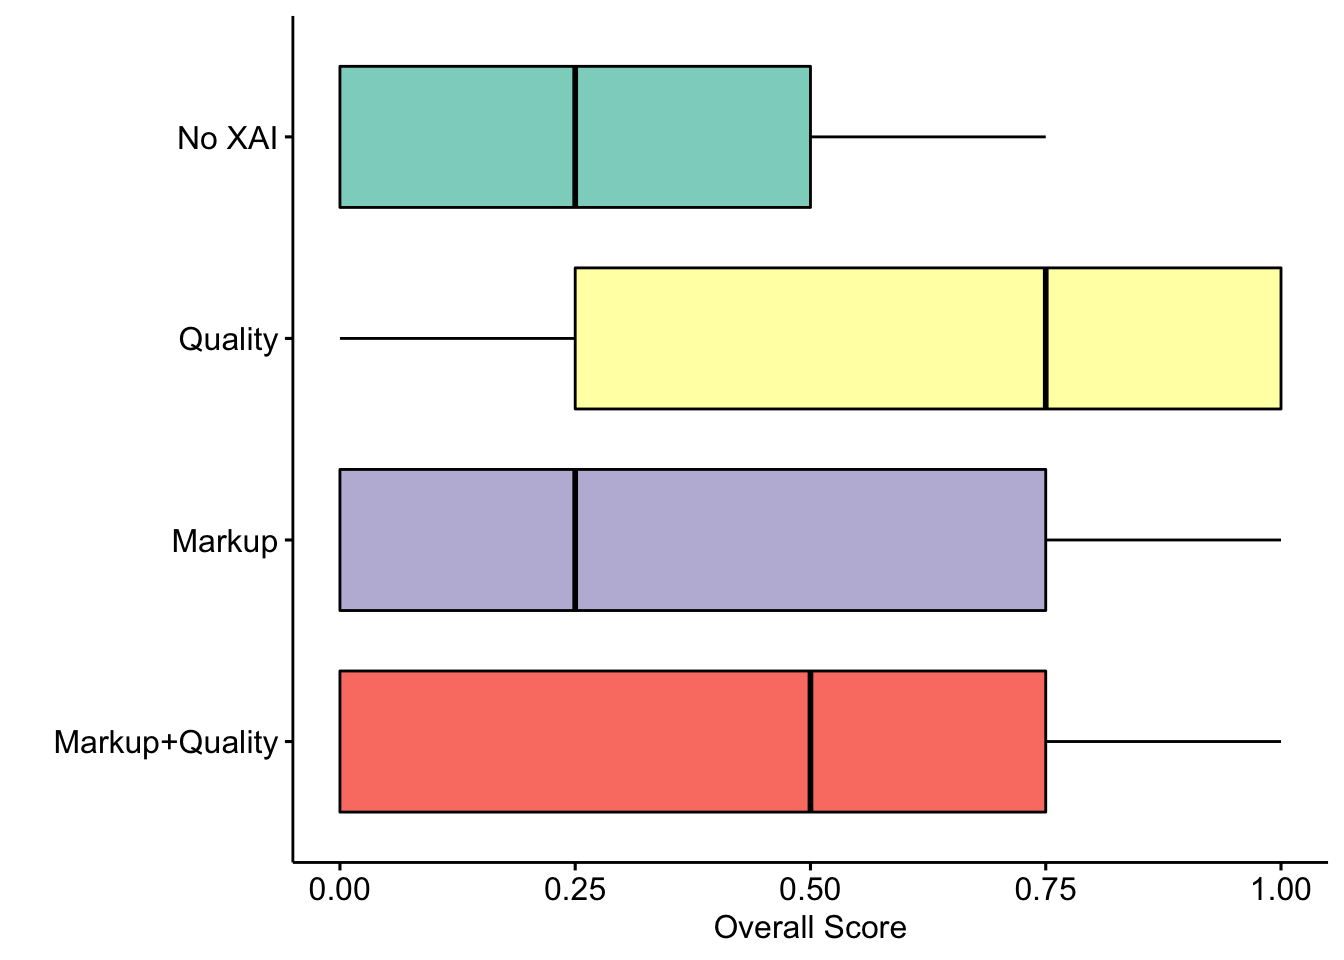
\includegraphics[width=0.50\textwidth]{exp1_overall_distribution.png}
    \caption{Boxplot of overall score by condition.}
    \label{fig:exp1_overall_distribution}
\end{figure}

These results suggest that showing sentence-level quality scores can significantly improve participants’ performance over No XAI, but word-level predicted errors on their own do not significantly affect performance. Therefore, we \textbf{partially accept H1.1}. The results also suggest that combining sentence-level quality scores and word-level predicted errors improves performance over No XAI and (though not significantly) improves performance over word-level predicted errors alone, therefore we \textbf{reject H1.2}.

\subsubsection{Does XAI affect trust?}

We asked participants before the experimental task “Please rate how much you trust artificial intelligence to correctly translate sentences from a language you do not speak into a language you do speak from 1 (No trust) to 5 (Complete trust).”  We asked the same question at the end of the experimental task. To analyze whether different conditions changed participant’s trust in machine translation, we calculated delta\_trust for each participant by subtracting their answer to the pre-experimental task trust question from their answer to the post-experimental task trust question. 
 
We ran a Kruskal-Wallis test of delta\_trust $\sim$ condition \footnote{We use a Kruskal-Wallis test because according to the Shapiro-Wilk Normality test delta_trust is not normally distributed ($W = 0.78, p < 0.001$).} and find no significant difference across conditions ($H(3) = 4.4, p = 0.22$). This suggests that neither the presence of XAI nor the different types of XAI significantly affected participants’ trust in machine translation, thus we \textbf{reject H2.1}. Average change in trust by condition is shown in Figure \ref{fig:exp1_delta_trust}.

\begin{figure}[h!]
    \centering
    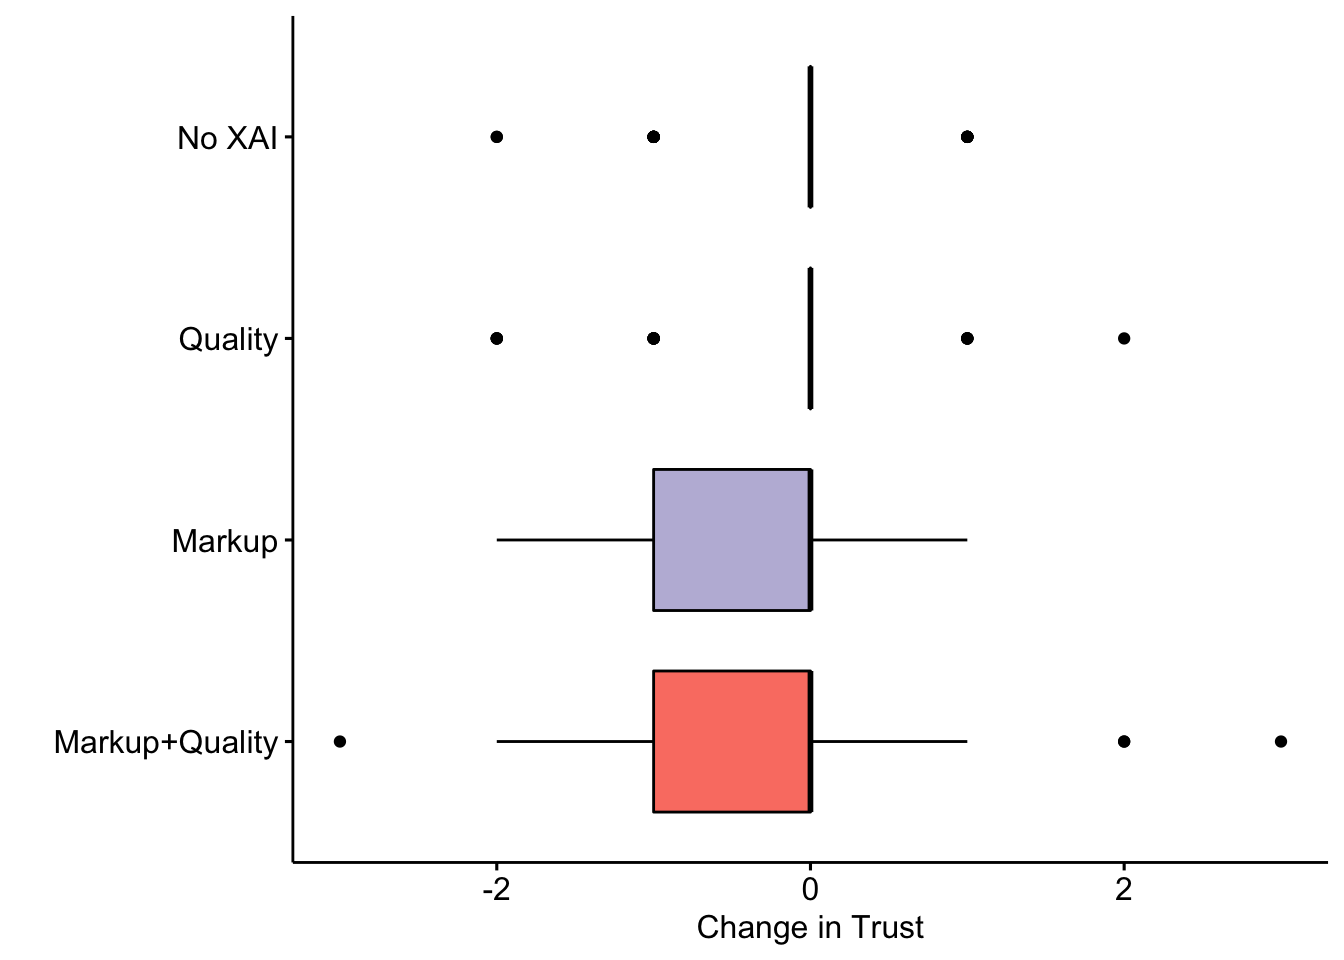
\includegraphics[width=0.50\textwidth]{exp1_delta_trust.png}
    \caption{Boxplot of change in trust by condition.}
    \label{fig:exp1_delta_trust}
\end{figure}

\subsubsection{Is the efficacy of XAI influenced by participants' individual differences?}

Prior work has shown that individual user differences can play a strong role in how well users utilize a visualization for a problem solving task\cite{liuSurvey2020}. However, there has been little research investigating how individual differences can affect understanding, trust, and use of AI. In an effort to start answering this question we captured three different individual differences of users (intolerance for ambiguity, usage of MT, and self-rated expertise) and analysed whether there were any correlations between these measures and users’ overall\_score. Our findings follow. 

\paragraph{Intolerance for Ambiguity} 

Given the survey instrument we use to measure Intolerance for Ambiguity\cite{gellerTolerance1993} participants’ scores could range from 7 (extremely low intolerance for ambiguity) to 49 (extremely high intolerance for ambiguity). The median score for intolerance for ambiguity of participants is 30. 

Within each condition we tested for a significant Pearson correlation between participants’ overall\_score and intolerance\_for\_ambiguity. Regression lines for each condition are shown in Figure \ref{fig:exp1_intol_ambiguity}. We find a significant correlation in the Markup condition ($r(53) = -0.27, p < 0.05$), and no significant correlation in any other condition (Quality -- ($r(57) = -0.14, p = 0.29$), Markup+Quality -- ($r(47) = -0.25, p = 0.08$), No XAI -- ($r(45) = -0.01, p = 0.95)$). This suggests that in the Markup condition as participants’ intolerance for ambiguity increases, their performance decreases, thus we \textbf{partially accept H3.1}. 

\begin{figure}[h!]
    \centering
    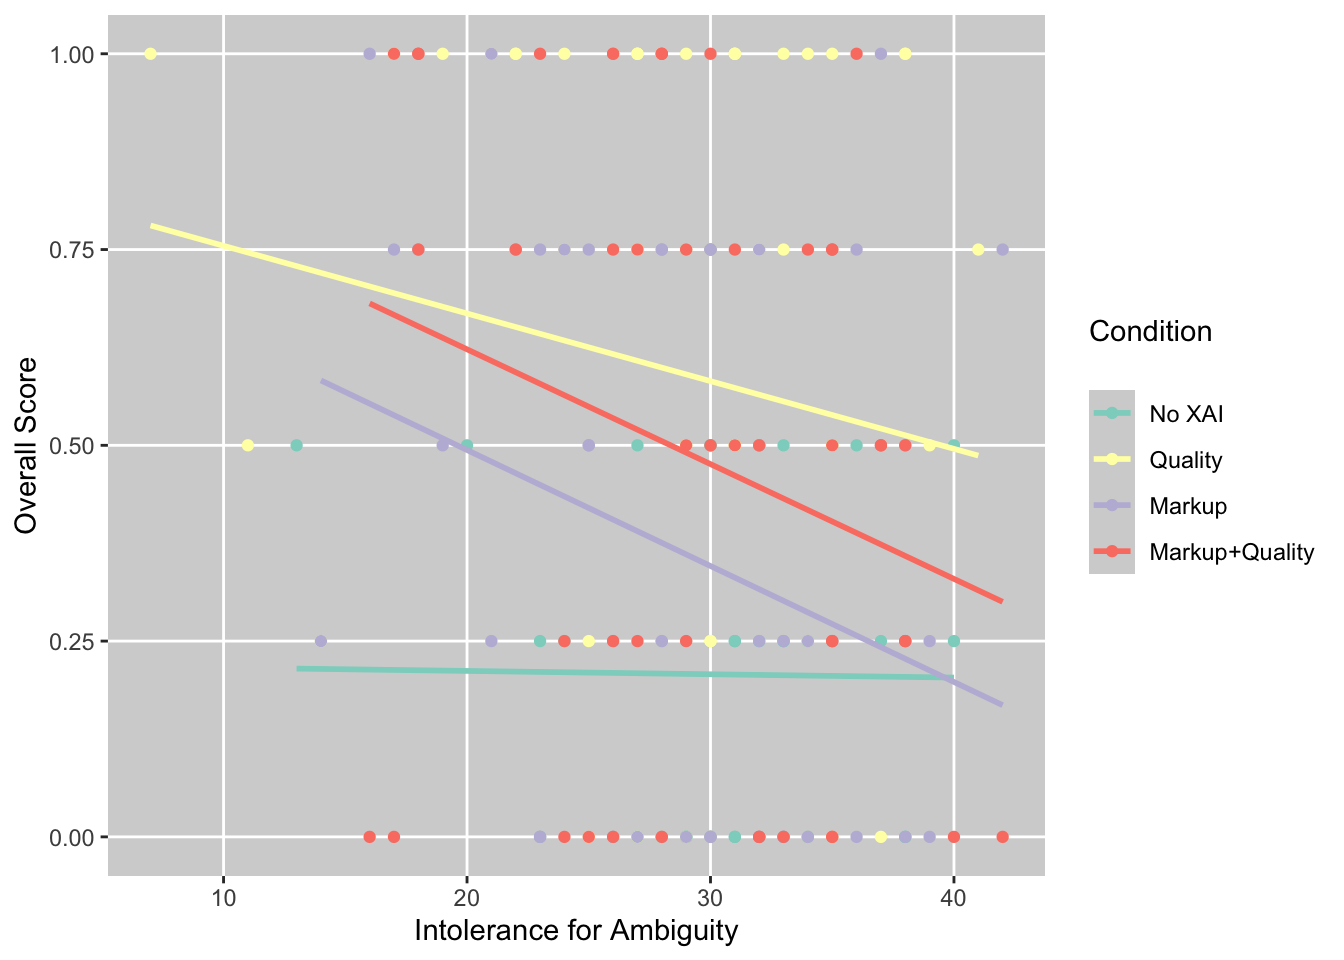
\includegraphics[width=0.50\textwidth]{exp1_intol_ambiguity.png}
    \caption{Regression lines of overall score and intolerance for ambiguity by condition.}
    \label{fig:exp1_intol_ambiguity}
\end{figure}

\paragraph{Usage of Machine Translation} 

We ask participants to rank how often they use Google Translate and Facebook Translate on a five-point scale of Never, Yearly, Monthly, Weekly, Daily. We assign weights to each point in the scale ranging from 1 (Never) to 5 (Daily) and use these to calculate a machine translation usage score for each participant. The higher this score, the more often a participant indicated using MT. 

Within each condition we test for a Pearson correlation between participants’ frequency of MT usage and performance. Regression lines for each condition are shown in Figure \ref{fig:exp1_MT_use}. We find a significant correlation between frequency of MT usage and overall score for participants in the Quality condition ($r(57) = -0.32, p < 0.05$), and no significant correlation in any other condition (Markup -- ($r(53) = -0.16, p = 0.26$), Markup+Quality -- ($r(47) = -0.20, p = 0.17$), No XAI -- ($r(45) = -0.23, p = 0.11$)). This suggests that in the Quality condition as participants’ frequency of MT usage increases, their performance decreases, thus we \textbf{partially accept H3.2}.

\begin{figure}[h!]
    \centering
    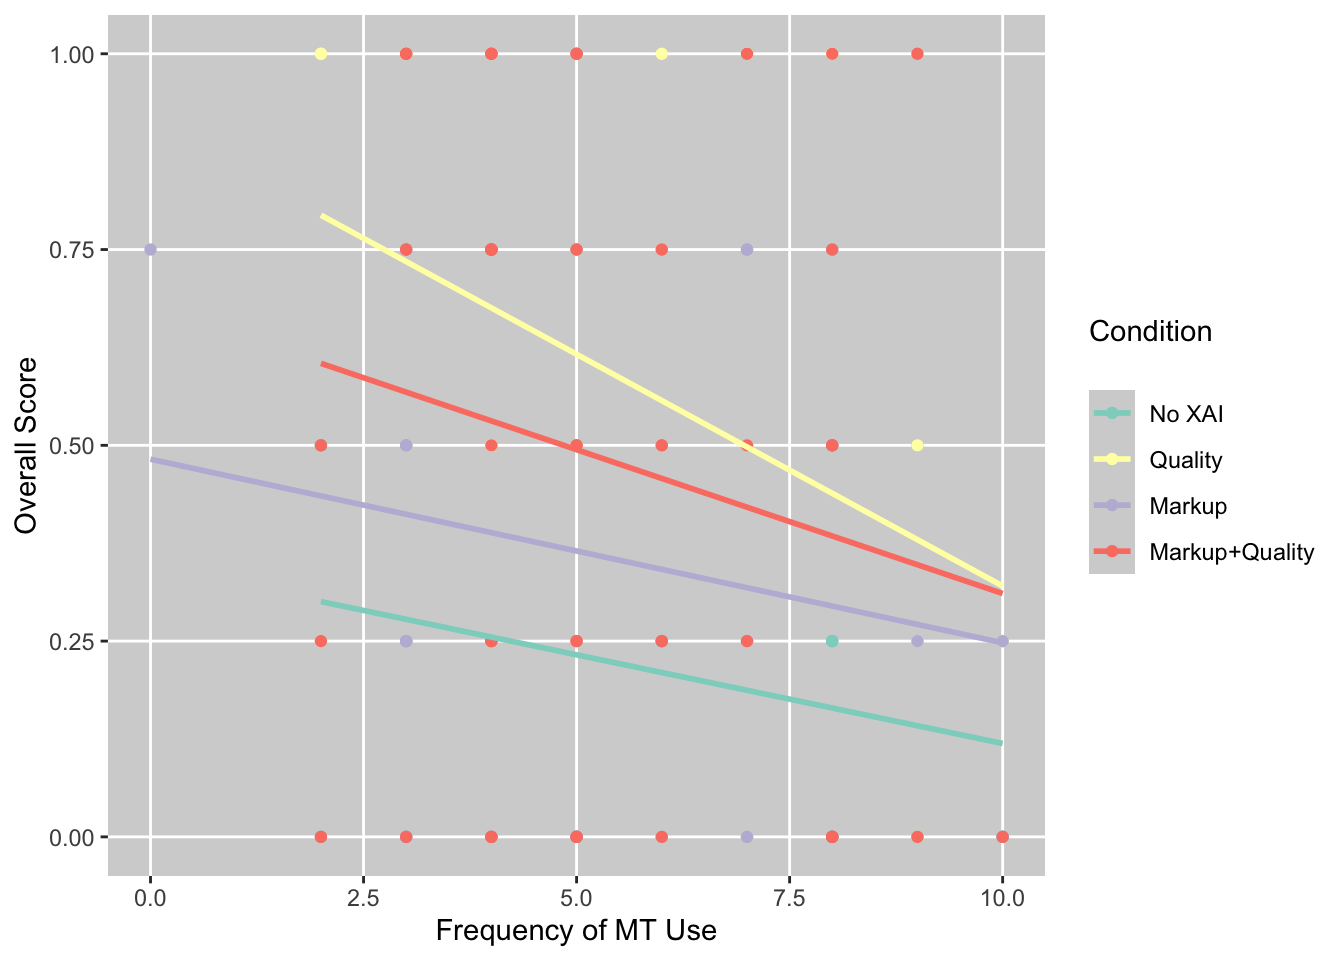
\includegraphics[width=0.50\textwidth]{exp1_MT_use.png}
    \caption{Regression lines of overall score and frequency of MT usage by condition.}
    \label{fig:exp1_MT_use}
\end{figure}

\paragraph{Self-rated Expertise}

We ask participants to rate their own expertise from 1 (Novice) to 5 (Expert) in four areas related to XAI: AI, MT, visualization, and statistics. We use these self ratings to test for correlations between participants’ self-rated expertise and performance. Regression lines for each condition are shown in Figure \ref{fig:exp1_expert}. 

\begin{figure}[h!]
    \centering
    
    \cbox{bar-noXai} \textit{No XAI} \quad
    \cbox{bar-Qual} \textit{Quality} \quad
    \cbox{bar-Markup} \textit{Markup} \quad
    \cbox{bar-MarkupQ} \textit{Markup$+$Quality}
    
    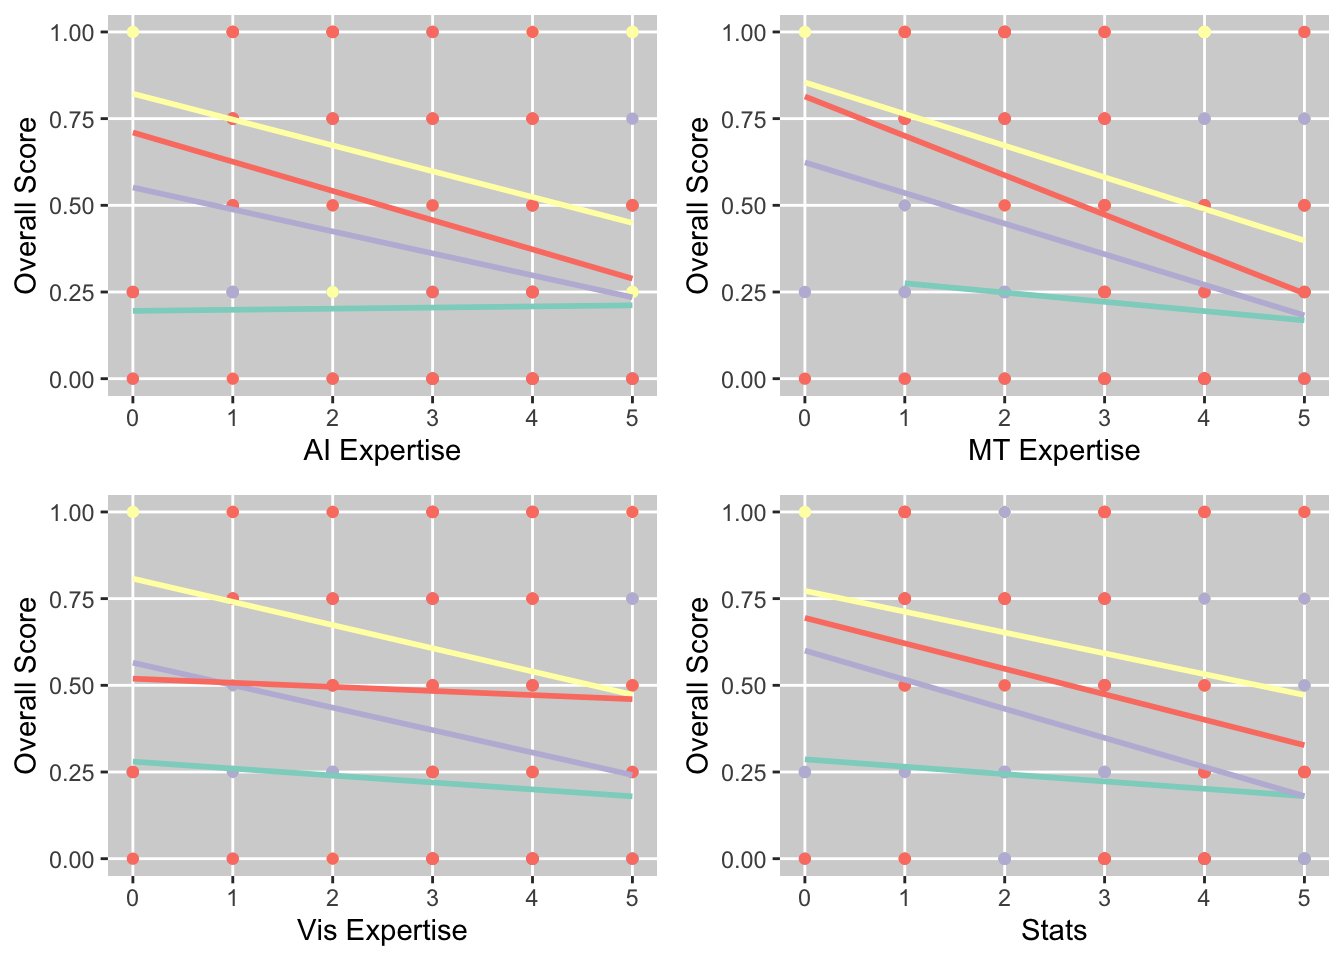
\includegraphics[width=0.50\textwidth]{exp1_expert.png}
    \caption{Regression lines of overall score and self-rated expertise by condition.}
    \label{fig:exp1_expert}
\end{figure}

Within each condition we test for a Pearson correlation between each self-rated expertise and overall score. In the Quality, Markup, and Markup+Quality conditions we find a significant correlations between self rated expertise in AI and MT and overall score. In addition, for participants in the Markup condition we find a significant correlation between self rated expertise in statistics and overall score. Analysis results are listed in Table \ref{tab:exp1_expertise_stats}. Overall, our results suggest that in all cases except for No XAI as self-rated expertise in AI and MT (and in the case of Markup statistics) increases, overall score decreases, thus we \textbf{partially accept H3.3}.

\begin{table}[]
\resizebox{0.80\textwidth}{!}{%
\begin{tabular}{llc}
\hline
\multicolumn{1}{c}{Measure}                            & \multicolumn{1}{c}{Condition} & Result                                   \\ \hline
\multirow{4}{*}{Self-rated expertise in AI}            & Quality                       & \textbf{r(57) = -0.27, p \textless 0.05} \\
                                                       & Markup                        & \textbf{r(53) = -0.27, p = 0.05}         \\
                                                       & Markup+Quality                & \textbf{r(47) = -0.32, p \textless 0.05} \\
                                                       & No XAI                        & r(45) = 0.02, p = 0.91                   \\ \hline
\multirow{4}{*}{Self-rated expertise in MT}            & Quality                       & \textbf{r(57) = -0.31, p \textless 0.05} \\
                                                       & Markup                        & \textbf{r(53) = -0.35, p \textless 0.01}          \\
                                                       & Markup+Quality                & \textbf{r(47) = -0.40, p \textless 0.01} \\
                                                       & No XAI                        & r(45) = -0.13, p = 0.39                  \\ \hline
\multirow{4}{*}{Self-rated expertise in visualization} & Quality                       & r(57) = -0.24, p = 0.06                  \\
                                                       & Markup                        & r(53) = -0.24, p = 0.07                  \\
                                                       & Markup+Quality                & r(47) = -0.04, p = 0.77                  \\
                                                       & No XAI                        & r(45) = -0.11, p = 0.48                  \\ \hline
\multirow{4}{*}{Self-rated expertise in statistics}    & Quality                       & r(57) = -0.21, p = 0.10                  \\
                                                       & Markup                        & \textbf{r(53) = -0.34, p \textless 0.05}          \\
                                                       & Markup+Quality                & r(47) = -0.26, p = 0.07                  \\
                                                       & No XAI                        & r(45) = -0.11, p = 0.46                  \\ \hline
\end{tabular}%
}
\caption{Pearson correlation results for each self-rated expertise measure by condition. Significant results are in \textbf{bold}.}
\label{tab:exp1_expertise_stats}
\end{table}

\subsection{Discussion of Findings} 

\ab{add headings / subsections?}

The main objective of this experiment is to test how different elements of MT XAI may (or may not) help users better understand and utilize MT output. Specifically, we test which elements of XAI help users identify which sentence in a passage is of low enough quality to warrant re-translation by a human. We find that participants are significantly more accurate at this task when they are shown sentence-level translation quality estimations (Quality condition), and sentence-level translation quality estimations alongside word-level predicted errors (Markup+Quality condition). Perhaps unsurprisingly, these results indicate that participants are significantly better at identifying which sentence in a passage is very poorly translated when XAI provides information on sentence-level quality. 

In addition, we find that providing word-level predicted errors (Markup) to users does not help them perform significantly better than providing no XAI. This finding highlights the importance of XAI design, particularly in what and how XAI designers show users. As shown here, though there are multiple ways to communicate information about MT quality (sentence-level quality and word-level quality), they are not equally useful to users. Our hope is that the outcome of this study not only informs what kind of quality estimations may be most useful for MT XAI, but more importantly that it demonstrates the importance of iterative, user-centered XAI design.

Given that an often cited goal of XAI is to moderate human trust in AI, we test whether different XAI interfaces have different effects on changing participants’ trust of MT. We find in general participants’ have high trust of MT \ab{add stats}, that does not change a lot throughout the course of the experimental task. Moreover, we find no significant differences in participants’ change in trust of MT given different XAI conditions. There are a few potential explanations for this. One is that participants in general come into the experiment with an appropriate amount of trust in MT quality. In this case, showing participants quality estimation for MT would help them perform the experimental task more accurately, but would not necessarily reveal to them that MT is less (or more) accurate than they already expected it to be. \ab{add some lit to support this? Or dig into the data some more and see if this related to how much people use google translate \& facebook translate?} 

Another explanation could be that our experimental task is not realistic enough to force users to consider their trust of MT output. Future work should explore a similar study in which the experimental task comes at more of a stake to the user. For example, asking the user to flag sentences as inappropriate based on MT, or asking the user whether or not they would repost a passage based on the MT. Scenarios such as these may elicit a stronger evaluation of trust from participants because the actions taken would be more directly tied to them. \ab{this is rambly, but I think I like where it’s going talking about study limitations and future work}

While we do not find that any individual differences affect participants’ performance across conditions, we do find in certain conditions some differences have an effect. For example, we find that in the Markup condition, there is a significant negative correlation between intolerance for ambiguity and performance. This could be because Markup is a very ambiguous way to communicate quality, in comparison to no indication (No XAI) and quality scores (Quality, Markup+Quality). With Markup, participants are left to themselves to determine what and how many word-level predicted errors indicate poor quality, as well as how to compare this metric between sentences. Quality scores, on the other hand, are clearly ordered and similarly summarize the quality of each sentence. Based on this result, we would recommend XAI designers focus on communicating quality through concise, comparable, and semantically meaningful methods, like quality estimation scores. 

In terms of MT usage, we find that in the Quality condition usage is significantly negatively correlated with performance. Similarly, we find that in all conditions except for No XAI that self-rated expertise in MT and AI is negatively correlated with performance. These findings are surprising, as we would expect people who are more familiar with MT through frequent usage to have a better understanding of its limitations and similarly we would expect people with more expertise in MT and AI to have a good understanding of MT limitations and of how to read and process quality indicators. We postulate that in both of these cases what we are observing is overconfidence leading to errors. We suspect that the more often one uses MT, the more the more familiar and comfortable they become with it and therefore see no need to rely on Quality scores instead of themselves to identify poor translations. We suspect that the same is true of self-rated experts in MT and AI, and the better someone thinks they are at understanding the underlying mechanisms of MT the more likely they are to want to rely on their own quality assessments instead of those shown by XAI. \ab{look for some sources to support this} Our findings suggest that novices are likely to follow XAI guidance, while those with more familiarity or expertise in the area are likely to ignore XAI guidance in favor of their own judgement. This means that in designing XAI interfaces, designers should pay specific attention to this population and center their design around the unique needs of these users instead of complete novices. \ab{Ab -- not in love with this takeaway…} 


 



